\documentclass[12pt,a4paper]{report}

\usepackage{styles/dolgozat}

\usepackage{listings}
\usepackage{styles/cpp}
\usepackage{styles/python}

\usepackage{hyperref}

\usepackage{dirtree}

\begin{document}

\pagestyle{empty} %a címlapon ne legyen semmi=empty, azaz nincs fejléc és lábléc

% A Miskolci Egyetem címere
{\large
\begin{center}
\vglue 1truecm
\textbf{\huge\textsc{Szakdolgozat}}\\
\vglue 1truecm

\includegraphics[width=4.8truecm, height=4truecm]{images/me_logo.png}\\
\textbf{\textsc{Miskolci Egyetem}}
\end{center}}

\vglue 1.5truecm %függõleges helykihagyás

% A szakdolgozat címe, akár több sorban is
{\LARGE
\begin{center}
\textbf{OBJ formátumú háromdimenziós modellek automatikus ellenőrzése és korrekciója}
\end{center}}

\vspace*{2.5truecm}
% A hallgató neve, évfolyam, szak(ok), a konzulens(ek) neve
{\large
\begin{center}
\begin{tabular}{c}
\textbf{Készítette:}\\
Boros Bence\\
Programtervező informatikus
\end{tabular}
\end{center}
\begin{center}
\begin{tabular}{c}
\textbf{Témavezető:}\\
Piller Imre
\end{tabular}
\end{center}}
\vfill
% Keltezés: Hely, év
{\large
\begin{center}
\textbf{\textsc{Miskolc, 2020}}
\end{center}}

\newpage


\newpage

\pagestyle{empty}

%Feladatkiiras
\begin{flushleft}
\textsc{\bfseries Miskolci Egyetem}\\
Gépészmérnöki és Informatikai Kar\\
Alkalmazott Matematikai Intézeti Tanszék\hspace*{4cm}\hfil \textbf{Szám:}
\end{flushleft}
\vskip 0.5cm
\begin{center}
\large\textsc{\bfseries Szakdolgozat Feladat}
\end{center}
\vskip 0.5cm
Boros Bence (EWE89T) programtervező informatikus jelölt részére.\newline

\noindent\textbf{A szakdolgozat tárgyköre:} Wavefront OBJ, fájlok beolvasása\newline

\noindent\textbf{A szakdolgozat címe:} \\
OBJ formátumú háromdimenziós modellek automatikus ellenőrzése és korrekciója\newline

\noindent\textbf{A feladat részletezése:}

\medskip

\emph{A WaveFront OBJ szabvány a leginkább elterjedt háromdimenziós objektum leírási módok közé tartozik. A szabványt a különböző megjelenítő és szerkesztő eszközök változatos mértékben támogatják. Az Interneten fellelhető modellek importálásánál ez gyakori problémát okoz.}

\medskip

\emph{A dolgozat célja egy olyan alkalmazás megtervezése és kifejlesztése, amely alkalmas OBJ fájlok elemzésére, és a benne lévő hibák javítására.}
\medskip

\emph{A dolgozatnak be kell mutatnia az OBJ szabvány lényeges elemeit. Részletezni kell a szöveges feldolgozás folyamatát. Külön ki kell térni a fájlokban előforduló gyakori problémákra, azok megoldási módjára. Az elkészült alkalmazás használatát példákkal illusztrálva be kell mutatni.}

\vfill

\noindent\textbf{Témavezető:} Piller Imre (egyetemi tanársegéd) \newline

% \noindent\textbf{Konzulens(ek):} (akkor kötelezõ, ha a témavezetõ nem valamelyik matematikai tanszékrõl való; de persze lehet egyébként is)\newline

\noindent\textbf{A feladat kiadásának ideje:}\newline

%\noindent\textbf{A feladat beadásának határideje:}

\vskip 2cm

\hbox to \hsize{\hfil{\hbox to 6cm {\dotfill}\hbox to 1cm{}}}

\hbox to \hsize{\hfil\hbox to 3cm {szakfelelős}\hbox to 2cm{}}

\newpage

\vspace*{1cm}  
\begin{center}
\large\textsc{\bfseries Eredetiségi Nyilatkozat}
\end{center}
\vspace*{2cm}  

Alulírott \textbf{Boros Bence}; Neptun-kód: \texttt{EWE89T} a Miskolci Egyetem Gépészmérnöki és Informatikai Karának végzős Programtervező informatikus szakos hallgatója ezennel büntetőjogi és fegyelmi felelősségem tudatában nyilatkozom és aláírásommal igazolom, hogy \textit{OBJ formátumú háromdimenziós modellek automatikus ellenőrzése és korrekciója}
című szakdolgozatom saját, önálló munkám; az abban hivatkozott szakirodalom
felhasználása a forráskezelés szabályai szerint történt.\\

Tudomásul veszem, hogy szakdolgozat esetén plágiumnak számít:
\begin{itemize}
\item szószerinti idézet közlése idézőjel és hivatkozás megjelölése nélkül;
\item tartalmi idézet hivatkozás megjelölése nélkül;
\item más publikált gondolatainak saját gondolatként való feltüntetése.
\end{itemize}

Alulírott kijelentem, hogy a plágium fogalmát megismertem, és tudomásul veszem, hogy
plágium esetén szakdolgozatom visszautasításra kerül.

\vspace*{3cm}

\noindent Miskolc, \hbox to 2cm{\dotfill} .év \hbox to 2cm{\dotfill} .hó \hbox to 2cm{\dotfill} .nap

\vspace*{3cm}

\hspace*{8cm}\begin{tabular}{c}
\hbox to 6cm{\dotfill}\\
Hallgató
\end{tabular}



\newpage

\noindent 1.

\begin{tabular}{cl}
&szükséges (módosítás külön lapon) \\
A szakdolgozat feladat módosítása& \\
& nem szükséges\\
&\\
\hbox to 4cm{\dotfill}&\multicolumn{1}{c}{\hbox to 5cm{\dotfill}}\\
dátum& \multicolumn{1}{c}{témavezető(k)}
\end{tabular}
\vskip1.5mm

\noindent 2. A feladat kidolgozását ellenőriztem:

\vskip1.5mm

\begin{tabular}{l@{\hspace*{4cm}}l}
témavezető (dátum, aláírás):& konzulens (dátum, aláírás):\\
\dotfill&\dotfill\\
\dotfill&\dotfill\\
\dotfill&\dotfill
\end{tabular}

\vskip1.5mm

\noindent 3. A szakdolgozat beadható:

\vskip1.5mm

\begin{tabular}{@{\hspace*{1.3cm}}c@{\hspace*{2.1cm}}c}
\hbox to 4cm{\dotfill}&\multicolumn{1}{c}{\hbox to 5cm{\dotfill}}\\
dátum& \multicolumn{1}{c}{témavezető(k)}
\end{tabular}

\vskip1.5mm

\noindent 4.
\begin{tabular}[t]{@{}l@{\hspace*{1mm}}l@{\hspace*{1mm}}l@{}}
A szakdolgozat& \hbox to 3.5cm{\dotfill} &szövegoldalt\\
              & \hbox to 3.5cm{\dotfill} &program protokollt (listát, felhasználói leírást)\\
              &\hbox to 3.5cm{\dotfill}   &elektronikus adathordozót (részletezve)\\
              &\hbox to 3.5cm{\dotfill} & \\
              &\hbox to 3.5cm{\dotfill} &egyéb mellékletet (részletezve)\\
              &\hbox to 3.5cm{\dotfill} &\\
\end{tabular}
\newline tartalmaz.

\vskip1.5mm

\begin{tabular}{@{\hspace*{1.3cm}}c@{\hspace*{2.1cm}}c}
\hbox to 4cm{\dotfill}&\multicolumn{1}{c}{\hbox to 5cm{\dotfill}}\\
dátum& \multicolumn{1}{c}{témavezető(k)}
\end{tabular}

\noindent 5.

\begin{tabular}{ll}
&bocsátható\\
A szakdolgozat bírálatra& \\
& nem bocsátható\\
\end{tabular}

\vskip1.5mm

\noindent A bíráló neve: \hbox to 8cm{\dotfill}

\vskip4mm

\begin{tabular}{@{\hspace*{1.3cm}}c@{\hspace*{2.1cm}}c}
\hbox to 4cm{\dotfill}&\multicolumn{1}{c}{\hbox to 5cm{\dotfill}}\\
dátum& \multicolumn{1}{c}{szakfelelős}
\end{tabular}

\noindent 6.
\begin{tabular}[t]{@{}l@{\hspace*{1mm}}l@{\hspace*{1mm}}l@{}}
A szakdolgozat osztályzata& &\\
&a témavezető javaslata:& \hbox to 3cm{\dotfill}\\
&a bíráló javaslata:& \hbox to 3cm{\dotfill}\\
&a szakdolgozat végleges eredménye:& \hbox to 3cm{\dotfill}
\end{tabular}

\vspace*{4mm}

\noindent Miskolc, \hbox to 4.5cm{\dotfill} \hspace*{2.5cm}
\begin{tabular}[t]{cc}
\hbox to 6cm{\dotfill}\\
a Záróvizsga Bizottság Elnöke
\end{tabular}


\cleardoublepage
\pagenumbering{gobble}
\tableofcontents
\cleardoublepage
\pagenumbering{arabic}

\newpage

\pagestyle{fancy}

\Chapter{Bevezetés}

Dolgozatom témáján sokat gondolkoztam, hogy vajon mi lenne a legmegfelelőbb számomra, mind saját elvárásaimmal kapcsolatban mind személyes fejlődésem érdekében. Fontosnak tartottam a választásommal kapcsolatban, hogy a témám legyen korszerű és legyen valamilyen grafikai vonatkozása.

Így végül konzulensemmel közös megállapodásra jutva a Wavefront OBJ formátumú modelleket javító szoftver elkészítésénél maradtunk. Ennek az eszköznek a megtervezése és elkészítése rendkívül izgalmas és sok érdekes programozási problémát rejt magában.

A dolgozatom feladatként egy olyan megoldás után kutatok a fent említett témakörön belül, mely segítségével elsősorban elemezni lehet a különböző OBJ fájlokat, de emelett meg is lehessen azokat jeleníteni, ráadásul lehetőség legyen  a javításukra is a programom használatával. A programom felhasználási területét tekintve elsősorban grafikus megjelenítőknél például játékszoftver  vagy különböző szimulátorok megvalósításánál lehetne hasznos.

Az alábbiak voltak a kitűzött célok a szoftverrek kapcsolatban.
\begin{itemize}
\item A szoftver könnyen átlátható és kezelhető legyen, az adott témában nem szakképzett
személy számára is.
\item Legyen elég komplex ahhoz, hogy  az igényeket maximálisan kiszolgálja.
\item Felhasználóbarát felülettel rendelkezzen, illetve a funkciók lehetőségekhez mérten egyszerűen elérhetők legyenek.
\end{itemize}

<<<<<<< HEAD
A dolgozatom elején rövid ismertetők formájában bemutatásra kerülnek a témához kapcsolódó fogalmak, mint a Wavefront által tervezett fájlformátum, anyagjellemzők, textúrák. Ezek mellett bemutatásra kerülnek a hasonló témakörben használatos szoftverek. Ezt követik a program irásához felhasznált különböző technológiák, majd a tervezés lépéseinek prezentálása és a program implementációjának részletes bemutatása, bemutatva a saját fejlesztésű \texttt{obj\_corrector\_tool} csomag felépítését és a program szerkezetét. Végül, a program tesztelésének bemutatása különböző fájlok felhasználásával zárja a dolgozatot.
=======
A dolgoztom elején rövid ismertetők formájában bemutatásra kerülnek a témához kapcsolódó fogalmak, mint a Wavefront által tervezett fájlformátum, anyagjellemzők, textúrák. Ezek mellett bemutatásra kerülnek a hasonló témakörben használatos szoftverek. Ezt követik a program irásához felhasznált különböző technológiák, majd a tervezés lépéseinek prezentálása és a program implementációjának részletes bemutatása, bemutatva a saját fejlesztésű \texttt{obj\_corrector\_tool} csomag felépítését és a program szerkezetét. Végül, a program tesztelésének bemutatása különböző fájlok felhasználásával zárja a dolgozatot.
>>>>>>> d90ab7ad850e6073308db2fb32cf995d4f8fdada

% A fejezet célja, hogy a feladatkiírásnál kicsit részletesebben bemutassa, hogy miről fog szólni a dolgozat.
% Érdemes azt részletezni benne, hogy milyen aktuális, érdekes és nehéz probléma megoldására vállalkozik a dolgozat.

% Ez egy egy-két oldalas leírás.
% Nem kellenek bele külön szakaszok (section-ök).
% Az irodalmi háttérbe, a probléma részleteibe csak a következő fejezetben kell belemenni.
% Itt az olvasó kedvét kell meghozni a dolgozat többi részéhez.


\Chapter{Koncepció}
% TODO: Le kellene írni az OBJ formátumról a fontosabb dolgokat!
\Section{OBJ fájlformátum}

Az OBJ fájlformátumot elsőnek a Wavefront Technologies kezdte kifejleszteni az 1980-as években az Advanced Visualizer animációs csomagjához. Ez a formátum egy olyan karakteres fájlformátum, ami utat enged geometriai objektumok leírásának egy aránylag egyszerű és egységes formában.\cite{martinreddy}

Magát a formátumot ott logikus használni, ahol egyszerű modelleket jelenítünk meg és ezeket nem akarjuk animálni. Például egy olyan egyszerű autó szimulátoros játéknál, ahol maga az autó geometriáját tekintve nem változik maximum a pozíciója és az orientációja, ezeket a transzformációs mátrix állításával egyszerűen megadhatjuk, így nincs szükség a modell animálására.\\

\noindent Wavefront obj fájlformátum:\\

\noindent A formátum általános felépítése a kevetkezőképpen alakul:

Minden sor áll egy kezdő karakterből vagy szimbólumból, utána egy elválasztójel (szóköz vagy tabulátor). Rögtön ezután szám vagy szöveg következik.\\

\noindent Minden karakter, ami egy kettőskereszt (\#) karakter után helyezkedik el, az egy megjegyzés:

\bigskip
\begin{python}
# ez egy megjegyzes
\end{python}
\bigskip
Geometriai vektorok:\\

\noindent \textbf{v} kezdőbetűvel ellátott sorok \textsl{geometriai vektort} definiálnak. Ezt követik (x, y, z [, w]) koordináták. A szögletes zárójel [ ] koordináta opcionális, alapértelmezés szerint 1.0 az értéke.
\bigskip
\begin{python} 
v -0,123 0,345 0,678 [1,0]
\end{python}
\newpage
\noindent Textúra koordináták:\\

\noindent \textbf{vt} kezdőbetűvel \textsl{textúra koordinátát} írunk le. Ezt (u, [, v, w]) koordináták követik, ezek 0 és 1 közötti értékek. A szögletes zárójel [ ] koordináta értékei opcionálisak és alapértelmezés szerint 0.0 az értékük.

\bigskip
\begin{python} 
vt 0.500 1 [0]
\end{python}
\bigskip
Normál vektorok:\\

\noindent \textbf{vn} kezdőbetűs sorok \textsl{normál vektort} definiálnak. Ezt  (x, y, z) koordináták követik.
\bigskip
\begin{python} 
vn -0.500 0.500 -0.500
\end{python}
\bigskip
Arcelemek:\\

\noindent \textbf{f} kezdőbetűvel egy \textsl{arc elemet} írunk le. Az \textsl{arc elemet} \textsl{geometriai vektor}, \textsl{textúra koordináta}, \textsl{normál vektor} indexek listájával írjuk le {/} jellel elválasztva. Vektor{\_}index {/} textura{\_}index {/}  normál{\_}index formátumban. Minden index 1-ről indul és növekszik annak sorrendjében, amelyben a hivatkozott elemet definiálták.\\

\noindent \textbf{Pár gyakran előforduló face definíció:}\\

\noindent Csak \textsl{geometriai vektorból} álló felület.
\bigskip
\begin{python} 
f v1 v2 v3 v4 ...
\end{python}
\bigskip
 Minden \textsl{geometriai vektorhoz} hozzá van rendelve egy \textsl{textúra koordináta} is.
\begin{python} 
f v1/vt1 v2/vt2 v3/vt3 ...
\end{python}
\bigskip
Minden \textsl{geometriai vektor} tartalmaz \textsl{textúra koordinátát} és \textsl{normál vektort}.
\bigskip
\begin{python} 
f v1/vt1/vn1 v2/vt2/vn2 v3/vt3/vn3 ...
\end{python}
\bigskip
A \textsl{geometriai vektorhoz} csak a \textsl{normál vektor} lett hozzárendelve, a \textsl{textúra koordináta} opcionális.
\bigskip
\begin{python} 
f v1/ /vn1 v2/ /vn2 v3/ /vn3 ...
\end{python}
\newpage
\noindentÖsszefoglalva, az OBJ formális nyelv kulcsszavakból (<\textbf{v}>, <\textbf{vt}>, <\textbf{vn}>, <\textbf{f}>), speciális karakterekből (<\textbf{/}>,<\textbf{\#}>) és számokból (<\textbf{Float}>, <\textbf{Integer}>) épül fel. Az OBJ nyelvtanát következő szabályokkal adhatjuk meg:\\

\noindent(OBJFájl) = {(Geometriai vektor)}+{(Textúra koordináta)}+{(Normál vektor)}+{(Arcelem)}\\
(Geometriai vektor) = (v)+(Float)+(Float)+(Float)\\
(Textúra koordináta) = (vt)+(Float)+(Float)+[0]\\
(Normál vektor) = (vn)+(Float)+(Float)+(Float)\\
(Arcelem) = (f)+{(Arc{\_}indexek)}\\
(Arc{\_}indexek) = (Integer)+[(/)+[(Integer)]+[(/)+[(Integer)]]]\\

\noindent A szögeltes zárójelbe [  ] foglalt elemek opcionálisak, vagyis a bennük lévő fogalom egyszer vagy egyszer sem jelenik meg a leírás során. \\

Wavefront formátum bemutatása példával, ez a példa egy szimpla négyszöget definiál:
\bigskip
\begin{python} 
v 0.0 0.0 0.0
v 1.0 0.0 0.0
v 1.0 1.0 0.0
v 0.0 1.0 0.0

vt 0.0 0.0
vt 1.0 0.0
vt 1.0 1.0
vt 0.0 1.0

vn 1.0 0.0 0.0 

f 1/1/1 2/2/1 3/3/1 4/4/1
\end{python}
\bigskip
A fájl először felsorolja a \textsl{geometriai vektorokat} (\textbf{v}), utána a \textsl{textúra koordinátákat} (\textbf{vt}) és \textsl{normál vektorokat} (\textbf{vn}), majd az \textsl{arcelemekkel} (\textbf{f}) egymáshoz rendeli ezeket. Ebben az esetben például a lapot négy csúcsponttal adtuk meg és {/} jellel elválasztva hozzá rendeltük a  \textsl{geometriai vektorok} , a \textsl{textúra koordináták} és a \textsl{normál vektorok} sorszámát.

A teljes OBJ formátum nagyon összetett, sok olyan szerkezeti egységet tartalmaz, ami egy szimpla objektum modellezéséhez szükségtelennek mondható.

\Section{Anyagjellemzők}

Az OBJ formátum 3D térben lévő objektumok csupán geometriáját írja le. Ezért szükségünk van még az anyagjellemzőkre is a képszintézis során. A különböző anyagokat fizikai jellemzőikkel írjuk le. Ezek a jellemzők például fényáteresztő képesség, fényvisszaverő képesség, törésmutató stb.\cite{diane1995mtl}\newpage
Ezeket a tulajdonságokat az MTL (Material Template Library) tartalmazza, a formátum hasonlóan az OBJ formátumhoz szintén szöveges. Az OBJ fájl tartalmazza a hivatkozást az {MTL} fájlra:
\bigskip
\begin{python}
mtllib fajlnev.mtl
\end{python}
\bigskip
Az \texttt{mtllib} hívja meg az MTL fájlt, ezután a \textsl{fájlnév} és a kiterjesztés következik \textsl{(.mtl)}.\\
OBJ fájlból akár egynél több anyagfájlra is lehet hivatkozni és egy MTL fájl tartalmazhat akár több anyagdefiníciót is.\\

\noindent A következő hívatkozással lehet beállítani a következő anyag anyagdefinícióját:
\bigskip
\begin{python}
usemtl (anyag neve)
\end{python}
\bigskip
Az anyag neve azonos egy anyagmeghatározással egy külső MTL fájlban.\\

\noindent Az objektumokat és sokszögcsoportokat a következő hivatkozások adják meg.
\bigskip
\begin{python}
o [objektum neve]
  ...
  g [csoport neve]
  ...
\end{python}
\bigskip
Sokszögek közötti árnyékolás a következővel állítható
\bigskip
\begin{python}
s 1
  ...
  s ki
  ...
\end{python}
\bigskip

\SubSection{MTL}
MTL fájl felépítése röviden:\\

Egy MTL ( Material Template Library) fájl tartalmazhat akár több anyagdefiníciót is. MTL fájl az anyagokat egymás után definiálja a fájlban, ezek a leírások \texttt{newmtl} paranccsal kezdődnek:
\bigskip
\begin{python}
newmtl szines
\end{python}
\bigskip
A \texttt{newmtl} egy új anyagot definiál, aminek a neve \texttt{"szines"}.
\newpage

\noindent A \textbf{Ka} kulcsszó az anyag ambient - környezettől független színét adja. Ez úgy viselkedik, mintha az anyag világítana, szóval ha a testet nem éri fény abban az esetben is ilyen lesz a színe. Viszont  az ambient tulajdonság nem viselkedik fényforrásként, attól hogy egy testnek ambient színe van az nem fogja megvilágítani a körülötte lévő többi testet. Az értéke RGB-ben van megadva 0 és 1 között.
\bigskip
\begin{python}
Ka 1.000 1.000 1.000
\end{python}
\bigskip
A \textbf{Kd} kulcsszó az anyag diffúz -  színét határozza meg. Ez a tulajdonság a test színét írja le, lényegében a diffúz tulajdonság meghatározza, egy felület rá eső fény mely részleteit nyeli el. Az értéke szintén RGB-ben van megadva 0 és 1 között.
\bigskip
\begin{python}
Kd 1.000 1.000 1.000
\end{python}
\bigskip
A \textbf{Ks} kulcsszó az anyag spekulár - színét adja. Ami az anyag tükröződéséért felelős. Értéke 0 és 1 között állítható. Amennyiben azt szeretnénk hogy az anyag minden ráeső fényt visszaverjen (tükörként működve), abban az esetben (1.0 1.0 1.0) értéket kell megadni ha pedig azt hogy mindet elnyeljen akkor (0.0 0.0 0.0) értékeket.
\bigskip
\begin{python}
Ks 1,000 1,000 1,000
\end{python}
\bigskip
Az \textbf{Ns} kulcsszó az anyag shininess - csillogását adja. Az anyagok felszíne nem csak tükörszerűen viselkedhetnek, hanem van saját fényük is. Ennek az értéke 0 és 1000 között határozható meg. Ezen skálán minél nagyobb értéket kap annál nagyobb lesz a fénysávok élessége.
\bigskip
\begin{python}
Ns 10.000
\end{python}
\bigskip
\Section{Textúrák}

Bár az OBJ fájl formátumnak nem része mégis fontos megemlíteni a textúrázást, a valóságszerű képek létrehozásánál egy fontos eszközünk a textúránk leképzése, hiszen a valóságban körülöttünk lévő tárgyak sem egyszínűek.

Textúrázás alatt általában kétdimenziós textúrázást értünk, de lehetnek ezek akár egy vagy háromdimenzionálisak is. A textúra geometriailag egy téglalap, ami sorokba és oszlopokba rendezet elemekből épül fel.

A textúra tehát adatok 1, 2 vagy 3 dimenziós tömbjének tekinthető. Az egyes textúra elemekhez tárolt adat képviselhet színt, fényerősséget vagy szín és alfa értékeket, azaz 1, 2, 3 vagy 4 adat  tartozhat minden textúra elemhez.

A téglalap alakú textúrákat azonban tetszőleges alakú sokszögekre, kell ráhelyezni. Ráhelyezést a modelltérben kell megadni, ezért  a textúráka is hatnak a modell- és vetítési transzformációk. Ennek érdekében az objektumok létrehozásakor a csúcspontok geometriai koordinátái mellett a textúra koordinátákat is meg kell adni, ezeknek a textúra koordinátáknak [0, 1] x [0, 1] egységnégyzeten belül kell elhelyezkedniük. \cite{juhasz2003opengl}
\Section{Modellbetöltő szofverek}

Manapság rengeteg modell elemző és betöltő szoftver áll rendelkezésünkre. A legtöbb ilyen szoftverről általánosságban elmondható, hogy ingyenes illetve  nyílt forráskóddal rendelkezik. Akadnak köztük elemzők online betöltők illetve telepítés után használható megjelenítők. Ezen szoftverek bemutatása következik.
\SubSection{Kixor modell elemző}

Az első ilyen elemző a Kixor modell elemzőszoftver volt.\cite{micah1987markup}\\
Elérési útvonal: \url{https://www.kixor.net/dev/objloader/}\\

A program futtatás után kielemezte a benne található \texttt{test.obj} fájlt \ref{fig:kixor}. ábra.
\bigskip
\begin{figure}[h]
\centering
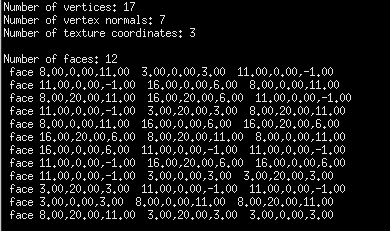
\includegraphics[scale=0.8]{images/kixor.png}
\caption{Kixor Elemző.}
\label{fig:kixor}
\end{figure}
\bigskip

\Aref{fig:kixor}. ábrán jól láthatóan módon a program elvégezte a szükséges számításokat majd visszatért a számított adatokkal.

Ez a szoftver nem alkalmas a modell megjelenítésére csak annak elemzésére viszont azt sok szemppontból megteszi, ha csak elemezni szeretnénk az OBJ fájlunkat abban az esetben kiváló lehetőségként szolgál.
\newpage
\SubSection{Online 3D Viewer}

Az első már megjelenítésre is alkalmas szoftver az Online 3D Viewer volt.\cite{online2014viktor}\\
Elérési útvonal: \url{https://3dviewer.net/}\\

Az oldalra érkezve \aref{fig:model_viewer1} ábran egy egyszerű és letisztult formátumot látunk, ahol rövid leírást ad a felhasználó számára, mik a támogatott fájlformátumok illetve azokat hogyan tudjuk megnyitni. 
\bigskip
\begin{figure}[h]
\centering
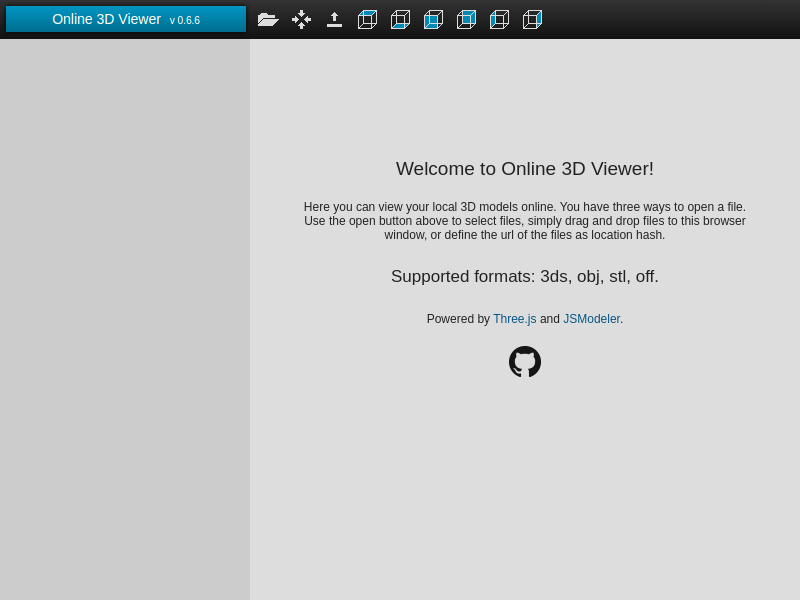
\includegraphics[width=\textwidth]{images/Model_Viewer.png}
\caption{Online 3D Viewer kezdőfelelület.}
\label{fig:model_viewer1}
\end{figure}
\bigskip

Mint \aref{fig:model_viewer1}. ábrán látható a számunkra lényeges \texttt{.obj} kiterjesztésű fájl formátum szintén a támogatott fájlformátumok között szerepel.

Leírásban benne van, hogy a megnyitás háromféleképpen történhet meg az oldal segitségével:
\begin{itemize}
\item Első lehetőségként az oldal bal felső részében található megnyitás gombra kattintva kiválasztjuk a megnyitni kivánt modellünket.
\item Második lehetőségként behúzzuk az oldalra a kívánt mdellünket egér segítségével.
\item Harmadik lehetőség pedig megadjuk a fájlok helyének webcímét.
\end{itemize}
\newpage
Miután kiválasztottuk a megfelelő objektumot az automatikusan megjelenik a rajzfelületen \aref{fig:model_viewer2} ábra.
\bigskip
\begin{figure}[h]
\centering
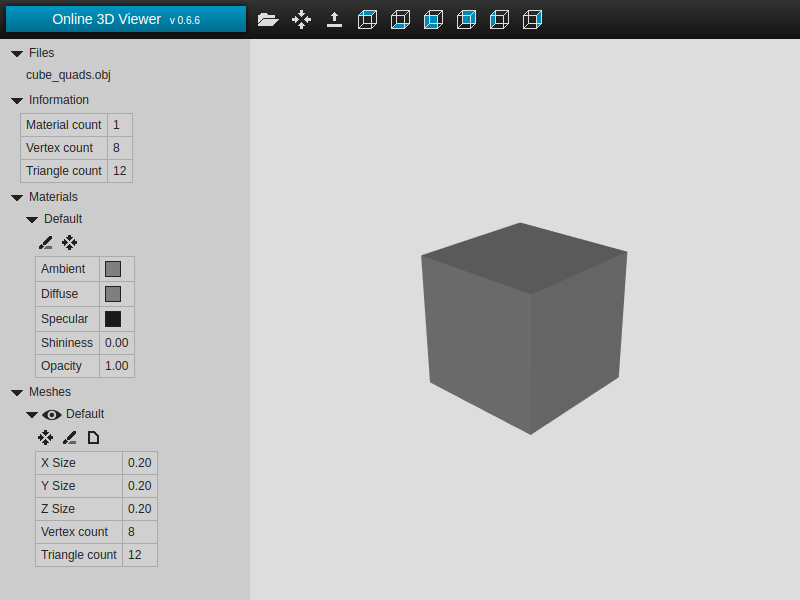
\includegraphics[width=\textwidth]{images/Model_Viewer_2.png}
\caption{Online 3D Viewer modell betöltéssel.}
\label{fig:model_viewer2}
\end{figure}
\bigskip

Rajzfelülettől balra találhatóak az objektumunkról gyűjtött adatok. Felette a model egyes síkidomjainak központba helyezése, a modellünk forgatása bal egérgomb folytonos nyomva tartásával és egér mozgatásával történhet. Ezen felül kameránk közelítése és távolítása görgő segítségével kivitelezhető.

A modellbetöltő gyors és egyszerű megjelenítést biztosít számunkra, tökéletesen működik a bonyolultabb geometriájú síkodomok megjelenítésével legyen szó háromszög, négyszög vagy akár ennél nagyobb csúcsszámmal rendelkező síkodomról. Ez nagy előnyt jelent felhasználó szempontból, amennyiben csak a modell megjelenítése a cél.

Sajnos kép alapú textúrázás nem támogatott a program által, ezért a textúrázás nem lehetséges. Másik probléma a szoftverrel, hogy egy időben csak egy OBJ file kirajzolására alkalmas.\\

Betöltő forráskódja illetve a programmal kapcsolatos rövid leírás megtalálható a következő weboldalon:

\url{https://github.com/kovacsv/Online3DViewer}
\newpage
\SubSection{Creators 3D Online Viewer}

Másik ilyen internetes betöltő a Creators 3D Online Viewer.\cite{creators2018creators3d}\\
Elérési útvonal: \url{https://www.creators3d.com/online-viewer}\\

\noindent Hasonlóan az előző Online 3D Viewer-hez a betöltő kezdőfelületén \aref{fig:3d1} ábra szintén tájékoztatást ad a támogatott fájlformátumokról.

Ez a betöltő is támogatja a OBJ fájl megjelenítését. A betöltő szintén támogatást nyújt a különböző sokaságú csúcspontal rendelkező síkidomok betöltésével, az előzőtől eltérően itt a megnyitás kétféle képpen történhet

\begin{itemize}
\item Első lehetőség: \\
A rajzfelültre húzzuk a megjelenítésre szánt objektum fájlunkat .
\item Második lehetőség:\\
Rajzfelületre kattintva megadjuk a fájlunk lokális helyének az útvonalát.\\
\bigskip
\begin{figure}[h]
\centering
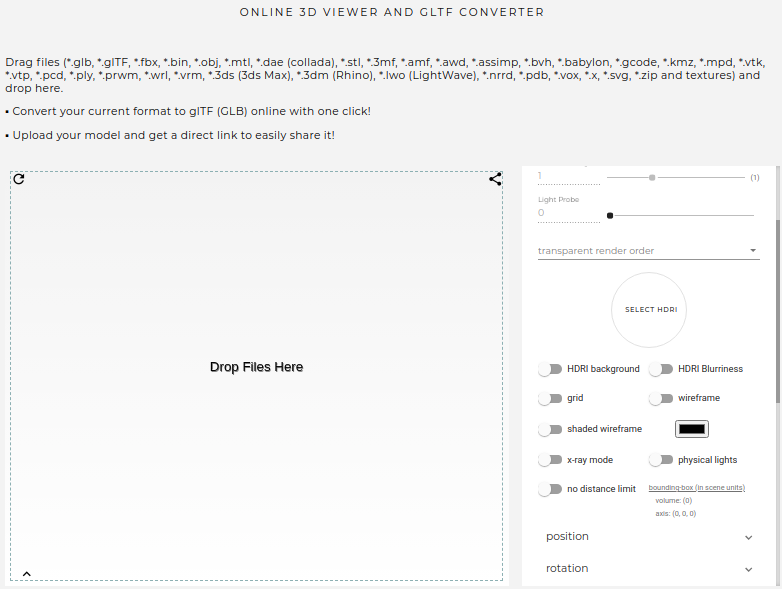
\includegraphics[width=\textwidth]{images/3D_creators.png}
\caption{Online 3D Viewer kezdőfelület.}
\label{fig:3d1}
\end{figure}
\bigskip

Rajzfelületre kattintva megadjuk a fájlunk lokális helyének az útvonalát.\\
\end{itemize}
\newpage
\bigskip
Amint kiválasztjuk a megjelenítésre szánt fájlunkat a felsorolt két lehetőség közül az objektum megjelenik a rajzfelületen \aref{fig:3d2}. ábra.
\bigskip
\begin{figure}[h]
\centering
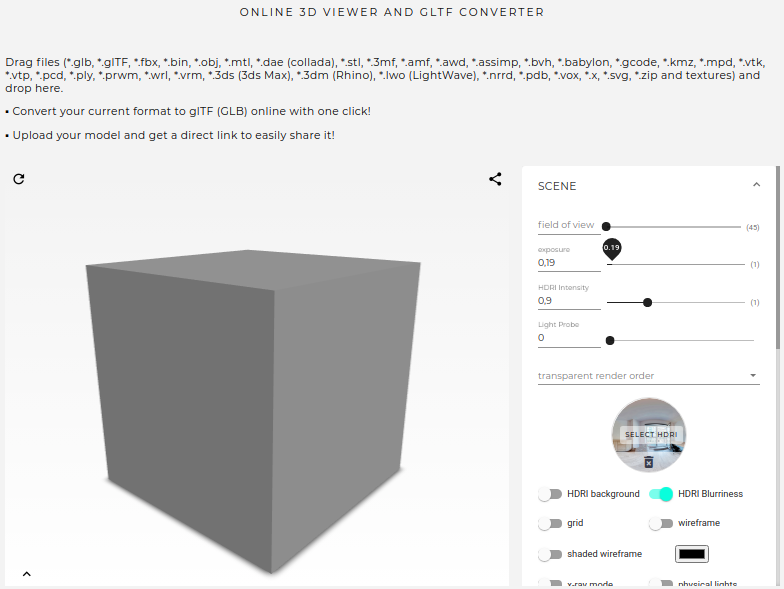
\includegraphics[width=\textwidth]{images/3D_creators_2.png}
\caption{Online 3D Viewer modell betöltéssel.}
\label{fig:3d2}
\end{figure}
\bigskip

Előző betöltőhöz hasonlóan szintén nagyon gyorsan megjelenítette a betöltésre szánt modellünket. Nyilván minél komplexebb a modellünk annál arányosabban több időbe telik a betöltés.

\newpage
Rajzfelülettől jobbra találhatóak különböző beállítások a megjelenítéssel kapcsolatban. Ilyenek például a keret kirajzolása (wireframe), aminek bekapcsolásával csak a modell hálója látszódik a \ref{fig:3d3}. ábrán.
\begin{figure}[h]
\bigskip
\centering
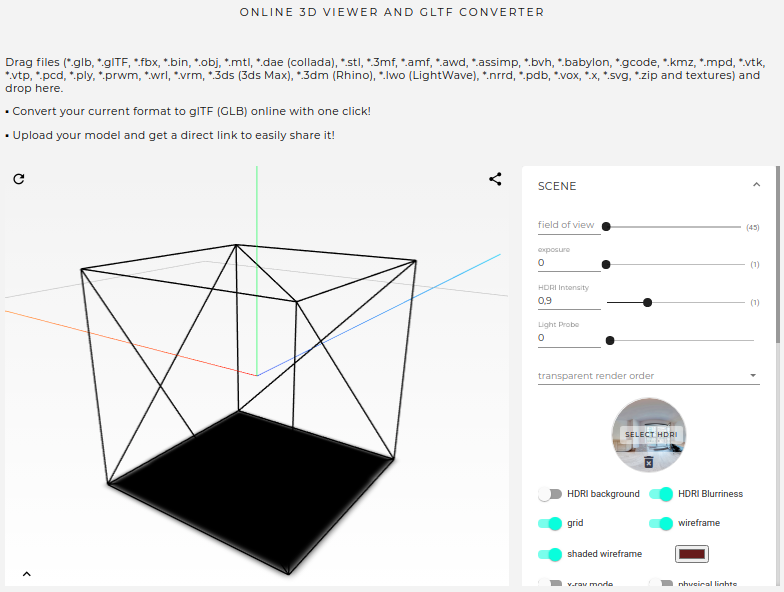
\includegraphics[width=\textwidth]{images/3D_creators_4.png}
\caption{Online 3D Viewer keret kirajzolással.}
\label{fig:3d3}
\end{figure}
\bigskip

De sok más egyéb funkcióval is ellátott például megjeleníthető koordináta tengely (grid), aminek segítségével vizsgálhatjuk az objektumunk irányultságát illetve elhelyeszkedését az x, y tengely kék és piros vonallal lettek jelezve a z tengely pedig zöldel  \ref{fig:3d3}. ábra.
\newpage
\SubSection{Model Loader}
Következő tesztelt szoftver, a Piller Imre által fejlesztett Model Loader volt.\cite{imre2020model}\\

\noindent A betöltő szoftverről részletes magyar nyelvű leírás és használati útmutató a következő webcímen található: \url{https://www.uni-miskolc.hu/~matip/grafika/}\\

A weboldalon található teljes dokumentáció beleértve : fejlesztő környezet beüzemelése, egyszerű objektumok kirajzolás, anyagjellemzők beállítása illetve textúrázás.

Ez a betöltő támogatja a kép alapú textúrázást, több objektum egy időben való betöltését  ezeket akár különböző textúrával illetve anyagjellemzővel is megjeleníthetjük.\\

Fejlesztői környezet beállítása után első futtatásra a \texttt{cube.obj} nevű példa a hozzátartozó textúrával következőképpen néz ki betöltés után (\ref{fig:model1}. ábra).
\bigskip
\begin{figure}[h]
\centering
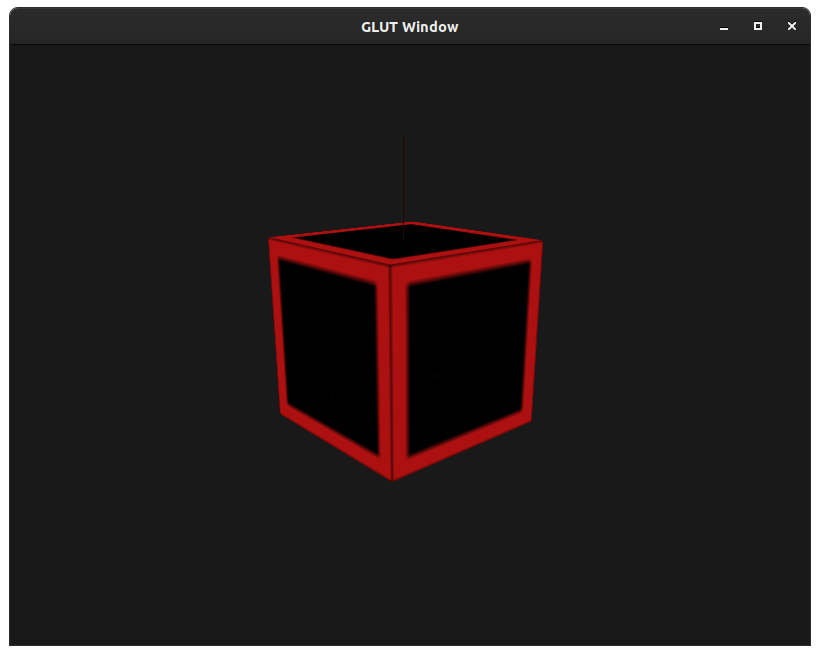
\includegraphics[width=\textwidth]{images/Model_loader.png}
\caption{Cube.obj megjelenítése.}
\label{fig:model1}
\end{figure}
\bigskip

Megjelenítés teljesen jól történt a megjelenítendő objektumot egy külön ablakban kirajzolta a program. A textúra illesztésével nem volt gond.\\
\newpage
Majd különböző komplexitású modellek betöltését teszteltem \ref{fig:modelbaby}. és  \ref{fig:modelbird}. ábrák.
\bigskip
\begin{figure}[h]
\centering
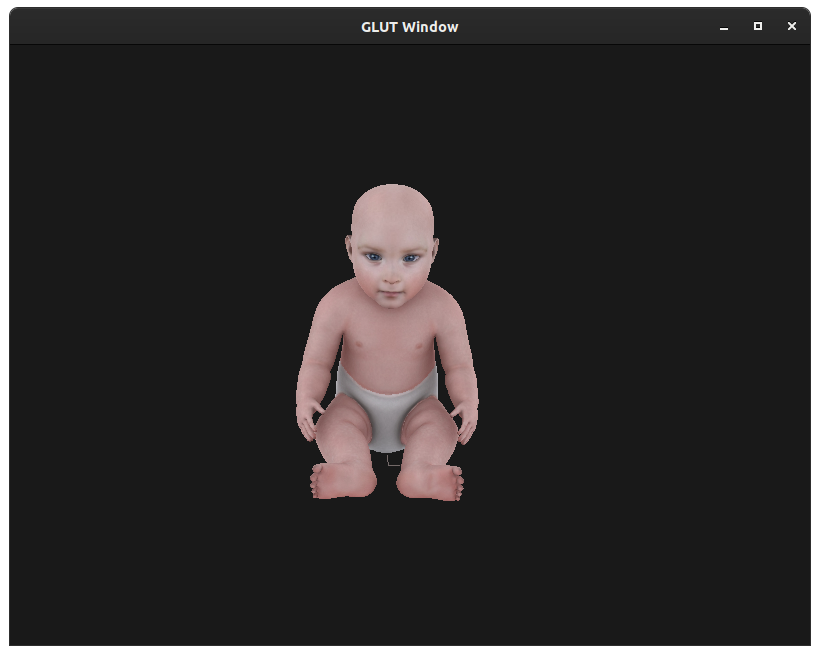
\includegraphics[scale=0.35]{images/model1.png}
\caption{Baby.obj modell megjelenítése.}
\label{fig:modelbaby}
\end{figure}
\bigskip
\begin{figure}[h]
\centering
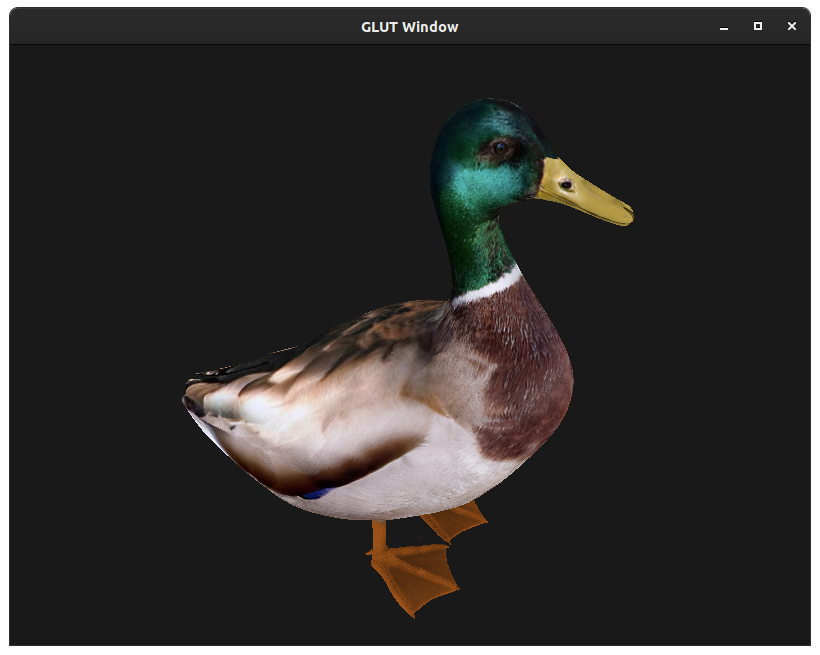
\includegraphics[scale=0.35]{images/bird.png}
\caption{Bird.obj modell megjelenítése.}
\label{fig:modelbird}
\end{figure}
\bigskip

Ezek a modellek szintén tökéletes megjelenítésre kerültek, a hozzájuk tartozó textúra betöltésével nem volt gond a modell megjelent a rajzfelületen.
\newpage
Pár ilyen betöltés után észrevettem,hogy a betöltő nem kezel háromszögnél nagyobb csúcspontal rendelkező síkidomokat,  \aref{fig:model1} ábra megjelenített \texttt{cube.obj} háromszögeit át konvertáltam négyszögekké, majd ezek után szintén betöltöttem a megjelenítőbe (betöltés \ref{fig:model2} ábra).
\bigskip
\begin{figure}[h]
\centering
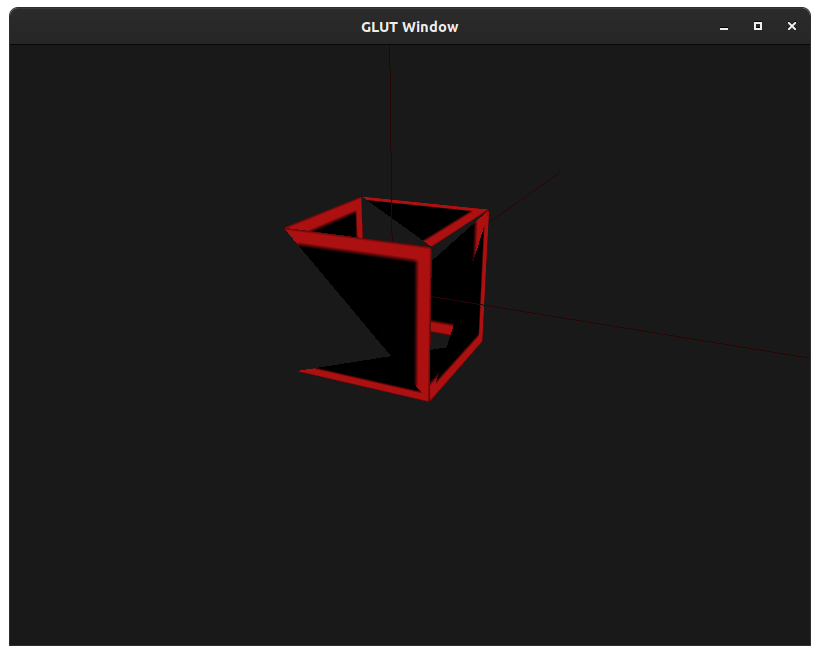
\includegraphics[width=\textwidth]{images/Model_quads.png}
\caption{Cube Model négyszögekkel.}
\label{fig:model2}
\end{figure}
\bigskip

Az ábrán jól látható hogy az objektum megjelent az ablakban viszont a kirajzolás nem megfelelő módon történt a kockánk eléggé hiányos, hiányzik a síkidomokról a negyedik csúcspont. A javító programunk egyik tervezett része ennek a hibának a javítására szolgál.
%\Section{Obj fájl formátum}
%\Section{Obj elemző szoftverek}
%\Section{Obj Bickbucket}
%\Section{Obj Bickbucket teszt}
\Chapter{Tervezés}
\Section{Modellek}

Modellek kapcsán első lépésben összegyűjtöttem számos OBJ file-t, egy részüknek az adatait \aref{fig:modellekt} táblázatban összegyűjtöttem.

\begin{table}[h]
\centering
\caption{Modellek táblázat}
\bigskip
\label{tab:modellek}
\begin{tabular}{|l|c|c|c|c|c|c|c|c|}
Modell neve& Vektor & T.vektor & N.vektor & Arc & H.szög & N.szög \\
\hline
baby.obj & 12030 & 13154 & 12030 & 12028 & 0 & 12028 \\
barrel.obj & 9348 & 9674 & 5411 & 5887 & 0 & 5880	\\
bird.obj & 8758 & 9582 & 8685 & 8752 & 0 & 8752 \\
boat.obj & 102669 & 203174 & 66538 & 100624 & 1294 & 99330\\
butterfly.obj & 1394 &	8328 &	0 & 2776 &	2776 &	0 \\
camera.obj & 17000 & 18580 & 16788 & 16984 & 0 & 16984 \\
cat.obj & 35290 & 36525 & 35014 & 35288 & 0 &	35288 \\
chair.obj & 78906 & 111336 & 45764 & 83074 & 11352 & 71722 \\
coral.obj & 43212 & 51349 & 43211 & 43200 & 0 & 43200 \\
cube.obj & 8 & 4 & 6 & 12 & 12 & 0 \\
deer.obj & 39402 & 41696 & 38642 & 39384 & 0 & 39384 \\
dog.obj & 35986 & 37096 & 35983 & 35984 & 0 & 35984 \\
dolphin.obj & 7338 & 7815 & 7337 & 7336 & 0 & 7336 \\
door.obj & 2058 & 2456 & 629 & 2152 &	220 & 1932 \\
lion.obj & 64558 & 67131 & 64556 & 64536 & 0 & 64536 \\
monkey.obj & 47490 & 49505 & 47490 & 47488 & 0 & 47488 \\
necklace.obj & 85592 &	94527 & 83931 & 85592 & 0 & 85592 \\
penguin.obj & 7494 & 7961 & 7493 & 7488 & 0 & 7488 \\
skull.obj & 40062 & 42682 & 40062 & 40728 & 1440 & 39288 \\
wrench.obj & 11568 & 13326 & 10508 & 11568 & 0 & 11568 \\
\hline
\end{tabular}
\label{fig:modellekt}
\end{table}

\Aref{fig:modellekt} tábázat modelleit a \url{https://free3d.com/} oldalról gyűjtöttem be. Ahol rengetek modell megtalálható. Ezeken a modelleken fellépő hibákat illetve különböző modellek kompatibilitási problémát vizsgáltam.\\

Vizsgálat során az  első szembetűnő dolog az volt, hogy ezek az objektumok komplexitásukban, jelentősen eltérnek egymástól. Voltak köztük olyan objektumok, amik viszonylag kevés komponensből állnak össze és voltak olyanok is, amik ezekhez képest jelentősen több elemből.
Természetesen az oldalon található modell fájlok többsége teljesen jól működik, de akadtak köztük hibásak is.\\

Majd rendszereztem őket az alábbi kategóriákba:
\begin{itemize}
\item Helyes modellek:\\
A megjelenítés tökéletesen megtörtént.
\bigskip
\item Javítható hibák:\\
A modellnek olyan javítható hibája van, ami a program segítségével majd javításra kerülhet.
\bigskip
\item Nem javítható hibák:\\
A modellnek olyan hibája van, ami nem kerülhet javításra a program segítségével.
\end{itemize}
\bigskip

\newpage

\Section{Saját Modell Struktúra Megtervezése}

\noindent Ennél a lépésnél megvizsgáltam és figyelembe vettem az általam vizsgált modell betöltők struktúrális felépítését és a következő konzekvenciát szűrtem le:\\

Az általam megvizsgált modellbetöltők tárolási módjai elég hasonlóak. Az objektum adataid egy közös modell struktúrában tárolják, ezt feltöltő adatokat pedig al struktúrákban.\\

A .obj model adatait egy közös model struktúrában tárolja a program a struktúrák egymás közötti felépítése \aref{fig:struct}-es ábrán látható.
\bigskip
\begin{figure}[h]
\centering
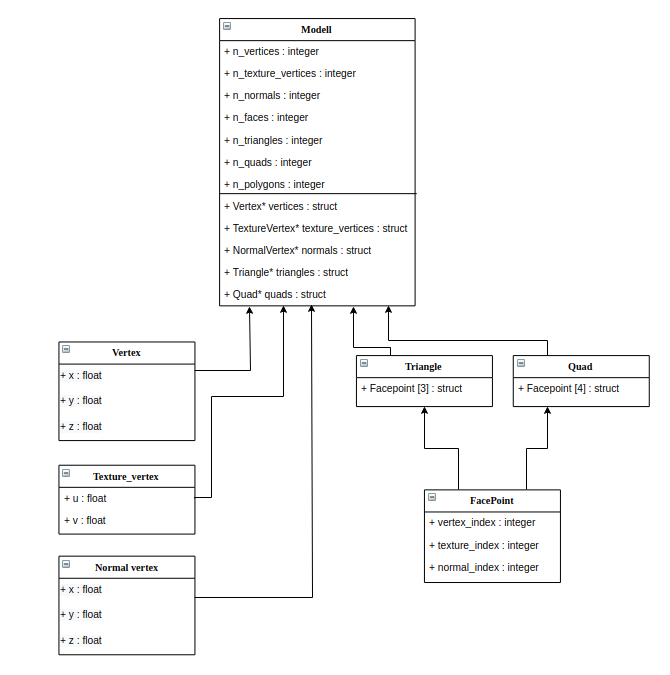
\includegraphics[width=\textwidth]{images/struct.png}
\caption{Model Struktúra.}
\label{fig:struct}
\end{figure}
\bigskip

Az integer típusú \texttt{n\_vertices}, \texttt{n\_texture\_vertices}, \texttt{n\_normals}, \texttt{n\_faces} illetve \texttt{n\_triangles}, \texttt{n\_quads} és \texttt{n\_polygons} változók feltöltésre kerülnek az OBJ fáj különböző változótípus darabasznámainak összeszámlálásával.
\begin{python}
typedef struct Model
{
    int n_vertices;
    int n_texture_vertices;
    int n_normals;
    int n_faces;
    int n_triangles;
    int n_quads;
    int n_polygons;
}Model
\end{python}
\bigskip

Ezt követően a \texttt{n\_vertices} számával közvetlen kiolvasásra kerülnek a \texttt{Vertex} struktúra különböző csúcspontjai.
\begin{python} 
typedef struct Vertex
{
    double x;
    double y;
    double z;
}Vertex;
\end{python}
\bigskip

Hasonlóan a Vertex struktúrához a \texttt{TextureVertex} csúcspontjai is kiolvasásra kerülnek az \texttt{n\_texture\_vertices} darabszámai.
\begin{python}
typedef struct TextureVertex
{
    double u;
    double v;
}TextureVertex;
\end{python}
\bigskip

Majd az előzőekhez hasonlóan a \texttt{NormalVertex}  struktúra csúcspontjai is feltöltődnek az \texttt{n\_normals} darabszámmal.
\begin{python}
typedef struct NormalVertex
{
    double x;
    double y;
    double z;
}NormalVertex;
\end{python}
\bigskip
\newpage
Végül a \texttt{Triangle} és \texttt{Quad} struktúrák is feltöltésre kerülnek, \texttt{FacePoint} struktúra segítségével.
\begin{python}
typedef struct FacePoint
{
    int vertex_index;
    int texture_index;
    int normal_index;
} FacePoint;

typedef struct Triangle
{
    struct FacePoint points[3];
} Triangle;

typedef struct Quad
{
    struct FacePoint points[4];
} Quad;
\end{python}
\bigskip

Az összes adat  \texttt{Model} struktúrában kerül eltárolásra ennek előnye, hogy egy közös, kap helyet az objektum összes fontos adata, így egyszerűbben lehet rájuk hivatkozni illetve a modellen történő szükséges változásokat  így könnyebben elvégezhetjük
\begin{python}
typedef struct Model
{
    int n_vertices;
    int n_texture_vertices;
    int n_normals;
    int n_faces;
    int n_triangles;
    int n_quads;
    int n_polygons;
    struct Vertex* vertices;
    struct TextureVertex* texture_vertices;
    struct NormalVertex* normals;
    struct Triangle* triangles;
    struct Quad* quads;
}Model;
\end{python}
\newpage
\Section{Elem indexelés}

\bigskip
\begin{figure}[h]
\centering
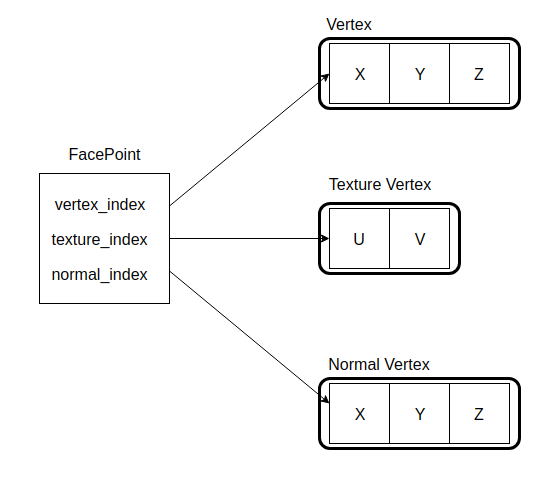
\includegraphics[scale=0.5]{images/point.png}
\caption{Model Struktúra.}
\label{fig:index_}
\end{figure}
\bigskip

\Aref{fig:index_} ábrán megtervezésre került egyes arcelemek hogyan fognak mutatni a különböző vektorok koordinátájra. Ennek a segítségével fogja a program összeállítani a sÍkodomokat a


%\Section{Betöltők tárolási módjai}
%\Section{Modellek}
%\Section{Saját modell struktúra}

\Chapter{Felhasznált Technológiák}
\Section{C programozási nyelv}
\begin{figure}[h]
\centering

\includegraphics[scale=0.6]{images/c_prog.png}
\caption{C programnyelv logo.}
\end{figure}
A C programozási nyelvet Dennis Ritchi és Ken Thompson az '70es évek elején fejlesztette ki. Általános célú programozási nyelvek közé tartozik, ami annyit tesz, hogy nem tartalmaz olyan nyelvi elemeket, amik kifejezetten egy bizonyos szakterület számára hoztak létre ellentében a szakterület specifikus nyelvekkel.\\

Kifejlesztésének elsődleges célja az volt, hogy  UNIX operációs rendszert könnyen hordozhatóvá tegyék több számítógép között.
Ennek oka az volt hogy a UNIX assembly nyelven készült hordohatóság nagyon nehézkes volt, a szerzők először olyan magasszintű programozási nyelvet kerestek, ami alkalmas operációs rendszerek írására,emellett mégis egyszerű és hardware programozásra alkalmas. Mivel olyan nyelvet nem találtak, ami minden kritériumnak megfelelő lett volna, ezért Ritchie Thompson létrehozta a C programozási nyelvet.\cite{brian1978thec}\\

Ezáltal a UNIX lett az első olyan operációs rendszer,melynek jelentős része magasszintű programozási rendszerben íródott.\\

UNIX-on kívül később számos más operációs rendszerre készítettek C fordítót, idővel piacvezető programozási nyelvek egyike lett.\\

\noindent Továbbfejlesztett változata a C++, ami már a C objektum orientált bővítése.
\newpage
\noindent C nyelv legfontosabb jellemzői:
\begin{itemize}
\item struktúrált:\\
Lényege hogy minden feladat olyan kis feladatra legyen felosztva, amelyek egymással nincsenek átfedésben.
\item  szabványos:\\
Minden felületen van fordítóprogramja és a fordítás egységes szabvánnyal történik.
\end{itemize}

A klasszikus "Hello World!" C programnyelven a program neve: \texttt{pelda.c }.
\bigskip
\begin{cpp}
#include <stdio.h>
 main()
 {
 printf("Hello World!\n");
 } 
\end{cpp}
\bigskip
Ennek a példának a fordítása gcc fordítóval történik
\begin{cpp}
gcc -o pelda pelda.c
\end{cpp}
\bigskip
Futtatás:
\begin{cpp}
./pelda
\end{cpp}
\bigskip
Kimenet:
\begin{cpp}
Hello World!
\end{cpp}
\bigskip
\SubSection{GCC fordító}
\bigskip
\begin{figure}[h]
\centering

\includegraphics[scale=0.6]{images/gcc.png}
\caption{GCC logója.}
\end{figure}
\bigskip
GCC a GNU Compiler Collection rövidítése. Szabadon elérhető C fordító Linux rendszerre, de már létezik Windows-ra elkészített változata is (mingw-n keresztül). A mingw egy szoftveres portja a GNU Compiler Collection-nek windows felületre.\cite{gnu2003richard}

\SubSection{PCRE}

Perl Compatible Regular Expressions rövidítve PCRE egy olyan C nyelven írt könyvtár, ami reguláris kifejezés motort valósít meg. Philip Hazel 1997-ben kezdte el kifejleszteni. Szintaxtisa erősebb és rugalmasabb mint a POSIX reguláris kifejezéseknek.\cite{philip1997pcre}


\Section{OpenGL}
\begin{figure}[h]
\centering

\includegraphics[scale=0.6]{images/opengl_logo.jpg}
\caption{OpenGL logója.}
\end{figure}
\bigskip
Open Graphics Library rövidítve OpenGL egy részletesen kidolgozott szabvány,amit  Silicon Graphics amerikai cég fejlesztett ki az 1990-es években. Ez egy olyan programozásra alkalmas felület, amely felületen keresztül grafikus kártya kezelése és 3D programozása megvalósítható.\cite{mason1999opengl}

Maga a felület több ezer különböző függvényhívásból áll, melynek segítségével a programozó közvetlenül a grafikus kártya vezérlésével 3D alakzatokat rajzolhatnak ki és ezek megvalósítását szabályozhatják közben. Felhasználása elég széleskörben zajlik használják: tervezésben/gyártásban, VR (virtuális valóság) létrahozatalában és szimulátorok esetében is.\\

Támogatott platformok többet között Linux és Windows, de használják még mobiltelefonokon illetve játékkonzolon.\\

Az első verzió 1992. június 30-án jelent meg, azóta az OpenGL-t számos alkalommal bővítették új verzió kiadásával.\\

Mára a legújabb verzió az OpenGL 4.6 , ami hatákonyabb geometria feldolgozás és árnyékoló végrehajtást illetve térbeli irányoktól függő eltolást biztosít a felhasználónak korábbi verziókhoz képest.\cite{khronos1997opengl}





%\Section{Felhasznált technológiák}


\Chapter{Javító szoftver megvalósítás}
A szoftver egy C nyelvű csomagként került megvalósításra, obj\_corrector\_tool (Objektum Javító Eszköz) névvel ellátva. A mappa tartalmazza az összes fájl-t a programhoz illetve az egységtesztekhez.\\

Csomag struktúrális felépítése a következő:
\bigskip
\dirtree{%
.1 /obj\_corrector\_tool.
.2 /include.
.3 bounding\_box.h.
.3 draw.h.
.3 model.h.
.3 \ldots.
.2 /OBJ.
.3 bird.
.4 bird.jpg.
.4 bird.obj.
.4 bird.mtl.
.4 \ldots.
.3 cube.
.4 cube.png.
.4 cube.obj.
.4 cube.mtl.
.3 \ldots.
.2 src.
.3 bounding\_box.c.
.3 draw.c.
.3 model.c.
.3 main.c.
.3 \ldots.
.2 tests.
.3 regex\_tests.h.
.3 test\_runner.c.
.2 Makefile.
}
\newpage
\texttt{Include} mappa tartalmazza a szükséges header állományokat.  \texttt{OBJ} almappáiban találhatóak a felhasznált OBJ fájlok. Az \texttt{src}-ben találhatóak a C nyelvű programfájlok. \texttt{Tests} mappában található Cmockában írt egységtesztek . Végül közvetlen az \texttt{obj\_\\corrector\_tool} található a \texttt{Makefile} .\\

\Section {Funkció hívás diagram}
\bigskip
\begin{figure}[h]
\centering
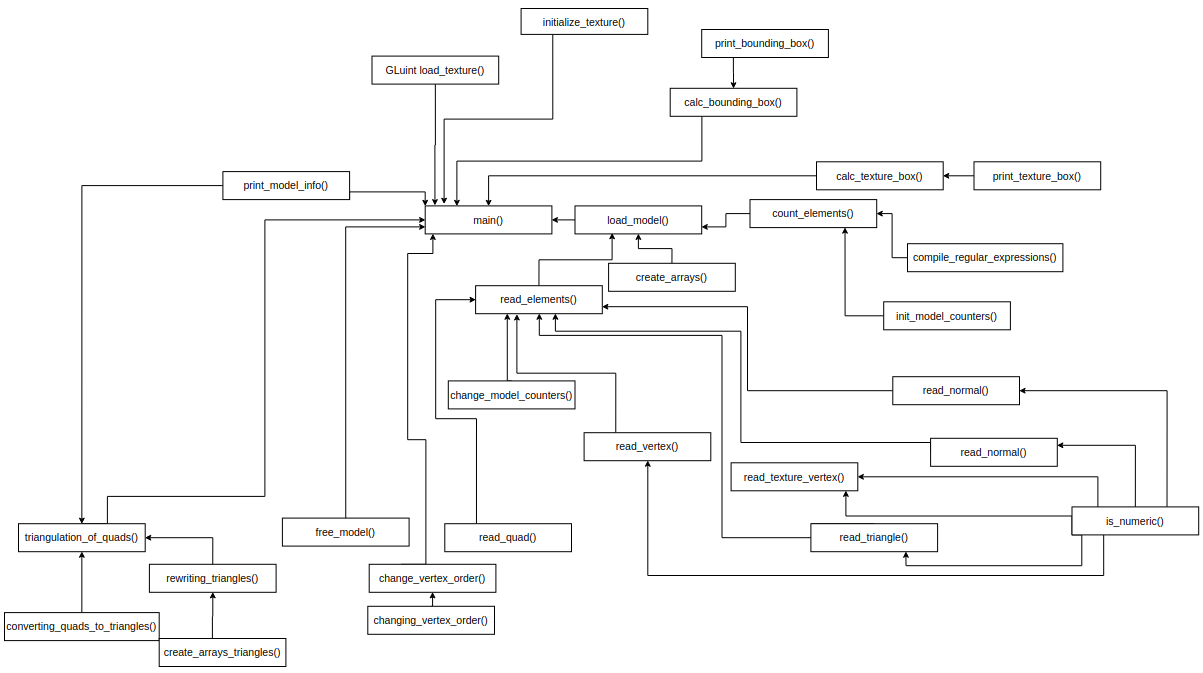
\includegraphics[width=\textwidth]{images/func.png}
\caption{Teljes Funkcióhívás Diagram.}
\label{fig:funk}
\end{figure}
\bigskip
\Aref{fig:funk} diagramon látható a program teljes funkcióhívás diagramja. Ez a diagram nagyon komplex és rengetek különálló funkciót kezel egyben. A különböző függvények egymást hívják meg a program futattása során végül az összes főbb funkció a \texttt{main} funkcióban találkozik.\\

Értelemszerűen, hogy egy OBJ javító alkalmazásról lévén szó az egyes funkciókat érdemes együtt  kezelni\\

Program főbb funkciói:
 \begin{itemize}
\item modell beolvasás
\item textúra beolvasás
\item hibák javítása
\item fájlba írás
\item megjelenítés
\end{itemize}
\bigskip
Feldolgozási folyamatot fentről-lefelé értelmezhetjük.
\newpage
\Section {Modell beolvasás}
Az alkalmazás minden olyan OBJ fájl betöltésére alkalmas, ami nem tartalmaz négyszögnél nagyobb csúcsszámmal rendelkező síkodomot, amennyiben az OBJ fájlunk tartalmaz ennél magasabb számút, azok számát képes összeszámlálni, viszont kezelni nem.\\

Elemzésre és javításra szánt OBJ fájl betöltése \texttt{main.c} (C nyelven írt programfájlon) belül \texttt{load\_model} függvénnyel történhet:
\bigskip
\begin{cpp}
load_model("utvonal/pelda.kiterjesztes", &model, &regular);
\end{cpp}
\bigskip

\texttt{utvonal}nál meg kell adni a fájl elérési útvonalát, majd a \texttt{pelda} helyére az OBJ fájlunk nevét majd a kiterjesztést (\texttt{.obj}).
\bigskip

\noindent Modell struktúra feltöltés bemutatása funkcióhívásokkal:\\

\texttt{Load\_model} beolvassa a megadott OBJ fájlt.
\bigskip
\begin{figure}[h]
\centering
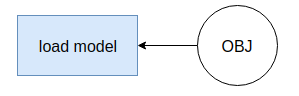
\includegraphics[scale=0.5]{images/load.png}
\end{figure}
\bigskip

Beolvasás után \texttt{count\_elements} összeszámolja \texttt{model} struktúra \texttt{n\_vertices},  \texttt{\\n\_texture\_vertices}, \texttt{n\_normals}, \texttt{n\_faces} illetve \texttt{n\_triangles}, \texttt{n\_quads} és \texttt{n\\\_polygons} egyes értékeit.
\bigskip
\begin{figure}[h]
\centering
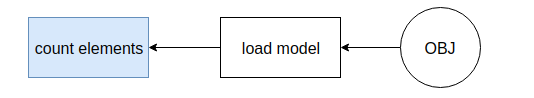
\includegraphics[scale=0.5]{images/count.png}
\end{figure}
\bigskip

Majd az összeszámolt értékek számával \texttt{create\_arrays} lefoglalja a szükséges nagyságú tömböket.
\bigskip
\begin{figure}[h]
\centering
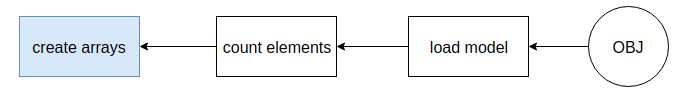
\includegraphics[scale=0.5]{images/create.png}
\end{figure}
\bigskip
\newpage
Ezután lefoglalt tömböt  a \texttt{read\_elements} kiolvassa a fájlból és feltölti az egyes értékekkel.
\bigskip
\begin{figure}[h]
\centering
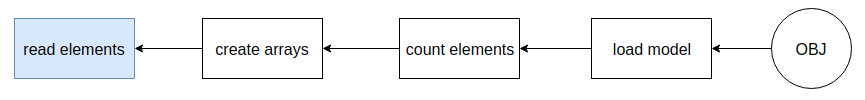
\includegraphics[scale=0.5]{images/read.png}
\end{figure}
\Section {Textúra}
Textúra pontok \texttt{u}, \texttt{v} [0 ; 1] intervallumon belül kell elhelyezkedni,ez az OBJ fájlok egy részében nem ígyvan ennek ellenőrzésére  a  \texttt{print\_texture\_box} nyújthat segítséget. Amennyiben utasítjuk a programot  a texture\_box kiszámítására és megjelenítésére, abban az esetben egy fix struktúrát jelenít meg számunkra a program és benne jelzi a számított adatokat.
\bigskip
\begin{python}
Texture box:
u in [0.000000, 1.000000]
v in [0.000000, 1.000000]
\end{python}
\bigskip

Balról jobbra haladva először megjeleníti a fájlban \textbf{u} legkisebb és legnagyobb értékét, majd ugyanezt megvalósítja a \textbf{v} koordináta számított adataival is.\\

Szoftver 2D (kép formátumú) textúrák megjelenítését támogatja  kívánt fájl megadása \texttt{texture.c} programfájlon belül \texttt{texture\_filename} után lehetséges.
\bigskip
\begin{cpp}
char texture_filename[] = "utvonal/pelda.kiterjesztes";
\end{cpp}
\bigskip

Saját képfájlunk megadásánál \texttt{utvonal} helyére a fájlunk elérési útvonala \texttt{pelda} helyére a képfájlunk neve \texttt{kiterjesztes} helyére pedig kiterjesztés kerül (\texttt{.jpg , .png, .tga}).
\Section {Megjelenítés}
Modellek mérete és elhelyezkedése nagy mértékben eltérő lehet. Ennek elemzése érdekében érdemes megnézni a \texttt{print\_bounding\_box} által számított adatokat és a kamerát ennek megfelelően pozíciónálni.
\bigskip
\begin{python}
Bounding box:
x in [-0.500000, 0.500000]
y in [-0.500000, 0.500000]
z in [-0.500000, 0.500000]
\end{python}
\bigskip

Ezen számok megadják, hogy az OBJ fájlunk mérete mekkora lesz a térben. Minden koordináta első száma a legkisebb második száma pedig a legnagyobb csúcs értékének elhelyezkedését adja az adott síkon.
\bigskip
\begin{cpp}
gluLookAt
(
        0.0, 0.0, -200, //eye (X, Y, Z)
        0.0, 0.0, 0.0,  //center (X, Y, Z)
        0.0, 1.0, 0.0 //up (X, Y, Z)
);
\end{cpp}
\bigskip

Kamera pozíciót a \texttt{gluLookAt} paraméterei állításával lehet pozícionálni.\\

Javító szoftver lévén maga a megjelenítő minimális funkciókkal lett ellátva, tehát nem tudjuk mozgatni  a modellünket, illetve kamera pozíciója sem változtatható megjelenítés után. Egyedül a modell forgatása lehetséges egér segítségével.\\

\texttt{house.obj} megjelenítése a hozzátartozó textúrával.(\ref{fig:demo} ábra)
\bigskip

\begin{figure}[h]
\centering
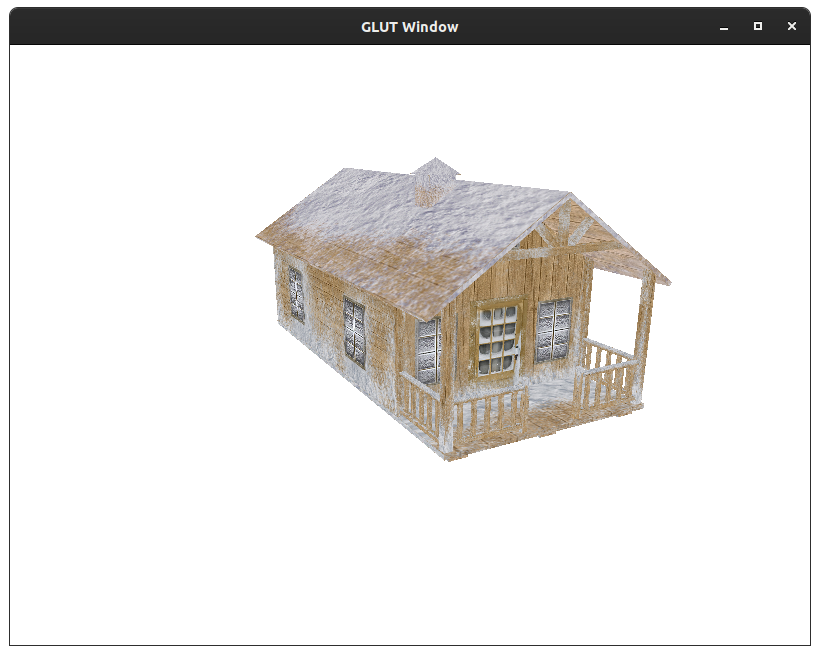
\includegraphics[width=\textwidth]{images/demo.png}
\caption{House.obj modell megjelenítés.}
\label{fig:demo}
\end{figure}
\newpage
\Section {Javítható hibák}
\SubSection{Háromszögesítés}
Korábbi észrevételeim alapján egyes betöltőknél gondot okoz, a háromszögeknél több csúcsszámú síkodomok kezelése, ennek a problémának a javítása fejlesztettem ki a \texttt{triangulation\_of\_quads} funkciót. Funkció célja, hogy négyszögeket két különálló  háromszögre bontjunk szét.
\begin{figure}[h]
\centering
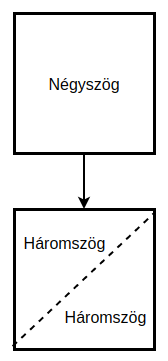
\includegraphics[scale=0.39]{images/triangulation.png}
\caption{Háromszögesítés elémletben.}
\label{fig:tri}
\end{figure}

\noindent A célünk ezzel, a \ref{fig:tri}. ábrán  látható módon minden négyszög síkodomot felbontsunk két különböző háromszögre szaggatott vonalon való metszéssel. Persze az ábrán látható négyszög egy szabályos négyzet, de ezek a négyszögek felvehetnek többféle alakzatot (téglalap, deltoid, rombusz stb...).

Ez úgy valósul meg, hogy a program kiválasztja az első beolvasott négyszöget az OBJ fájlból annak első három csúcs koordinátájából képez egy háromszöget majd a következő háromszöget az előző négyszög első harmadik, illetve negyedik koordinátájából képezi le így végighaladva az összes négyszögön ami az OBJ fájlunkban található.\\Ennek szemléletetése a \ref{fig:tri1}. ábrán látható.
\begin{figure}[h]
\centering
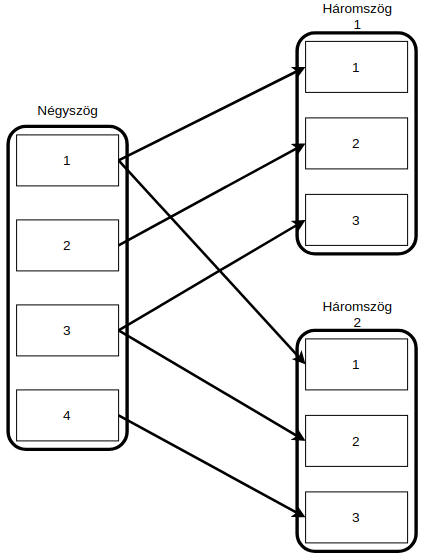
\includegraphics[scale=0.39]{images/haromszog.png}
\caption{Háromszögesítés diagram.}
\label{fig:tri1}
\end{figure}
\newpage

Megvalósítás során \texttt{triangulation\_of\_quads} funkció modell struktúránkból elveszi az összes négyszöget és két háromszöggel tölti fel azok helyét, illetve a lapok számát is növeli minden felvágott négyszög esetében eggyel.

\begin{figure}[h]
\centering
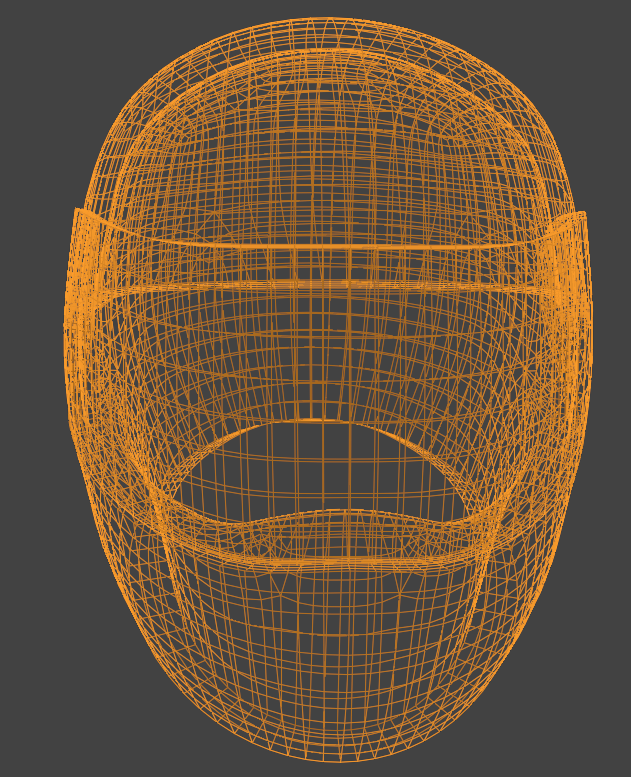
\includegraphics[scale=0.32]{images/helmet1.png}
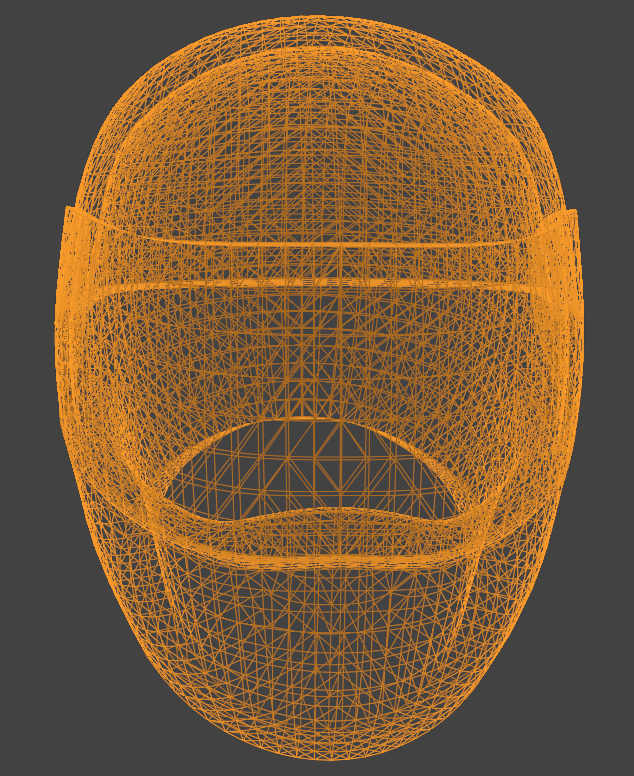
\includegraphics[scale=0.32]{images/helmet2.png}
\caption{helmet.obj háló.}
\label{fig:tri2}
\end{figure}

Az \ref{fig:tri2}. ábra bal oldali képen az eredeti \texttt{helmet.obj} modell látható, a modell hálójának megjelenítésével, a jobb oldali képen pedig már a háromszögelt változat. Jól láthatóak az eltérések a két modell rajzolt állapota között.
\begin{table}[h]
\centering
\caption{helmet.obj adatait tartalmazó táblázat}
\bigskip
\label{tab:modellek}
\begin{tabular}{l|c|c|}
& helmet.obj & helmet.obj háromszögesítés után \\
\hline
geometria csúcsok & 6066 & 6066 \\
textúra koordináták & 6409 & 6409 \\
normál csúcsok & 6650 & 6650 \\
lap elemek & 6064 & 12128 \\
háromszögek & 0 & 12128 \\
négyszögek & 6064 & 0 \\
\hline
\end{tabular}
\label{fig:tri3}
\end{table}

Az \ref{fig:tri3}. összesítő táblázat megmutatja hogyan változtak a \texttt{helmet.obj} adatai a háromszögesítés után. Láthatóan az összes négyszög eltünt a modellből ezeket két háromszögre bontotta a szoftver, az lap elemek száma is duplájára nőtt.
\newpage
\SubSection{Bejárási irány megváltoztatás}
\bigskip
A program ezen része arra szolgál, hogy a háromszögeink bejárási irányát meg tudjuk változtatni \aref{fig:bej1}. ábrán látható módon.
\bigskip
\begin{figure}[h]
\centering
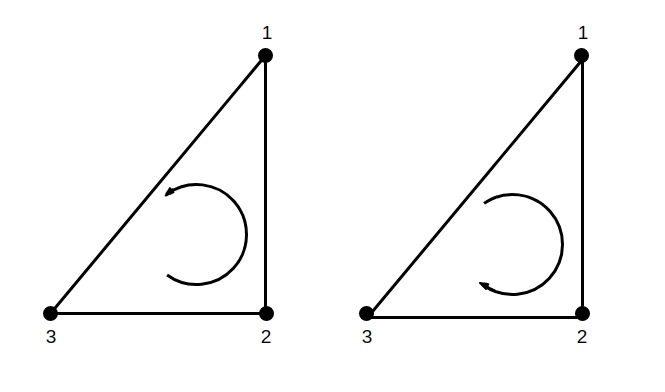
\includegraphics[scale=0.5]{images/bejarasi.png}
\caption{Bejárási irány változtatás elméletben.}
\label{fig:bej1}
\end{figure}
\bigskip

Egy háromszög csúcsok közötti bejárást kétféleképpen tudjuk bejárni. \Aref{fig:bej1}. ábrán bal oldalt látható  óramutató járásával ellentétes bejárási sorrendben (1 -> 3 -> 2), amit a megjelenítőnk alapból használ, jobb oldalon pedig az ellenkezője óramutató járásával megegyező bejárás (1 -> 2 -> 3).

Ez a funkció \texttt{change\_vertex\_order} függvény néven van a programba implementálva. Amennyiben úgy döntünk és ezt alkalmazzuk a programunk elvégzi a bejárási irány cserét model struktúrába betöltött objektomunkon.

Megjelenítés során a megjelenítő ugyanúgy óramutatójárásval ellentétesen fogja megjeleníteni a modellünket, viszont a programunk \texttt{change\_vertex\_order} függvény segítségével megváltoztatta csúcsok sorrendjét így a megjelenítés már óramutató járásával megegyező módon fog történni az eredeti OBJ fájlhoz képest.\\
\newpage
\Aref{fig:bej2}. ábra egy egyszerű modellen keresztül ezt hivatott bemutatni.
\bigskip
\begin{figure}[h]
\centering

\includegraphics[scale=0.5]{images/order.png}
\caption{Bejárási irány hiba.}
\label{fig:bej2}
\end{figure}
\bigskip

Jól látható módon a felső modellünk hibásan az alsó pedig jól került megjelenítésre. Két modell összesen az lapok közötti bejárási útvonal a különbség a két modell összes többi csúcsa ugyanaz \aref{fig:bej3} táblázatban bemutatásra kerül a két objektum közti eltérés. Ez a táblázat csak az lapok közötti eltérést mutatja.

\newpage

\begin{table}[h]
\centering
\caption{Lap elemeket összehasonlító táblázat}
\bigskip
\begin{tabular}{|c|c|}
Felső modell& Alsó modell \\
\hline
f  1//1 2//2 3//3 & f  1//1 3//3 2//2 \\
f  1//1 3//3 4//4 & f  1//1 4//4 3//3 \\
f  5//5 6//6 7//7 & f  5//5 7//7 6//6 \\
f  5//5 7//7 8//8 & f  5//5 8//8 7//7 \\ 
f  1//1 2//2 6//6 & f  1//1 6//6 2//2 \\
f  1//1 5//5 6//6 & f  1//1 6//6 5//5 \\
f  1//1 4//4 8//8 & f  1//1 8//8 4//4 \\
f  1//1 5//5 8//8 & f  1//1 8//8 5//5 \\
f  3//3 6//6 7//7 & f  3//3 7//7 6//6 \\
f  2//2 3//3 6//6 & f  2//2 6//6 3//3 \\
f  3//3 8//8 7//7 & f  3//3 7//7 8//8 \\
f  3//3 4//4 8//8 & f  3//3 8//8 4//4 \\
\hline
\end{tabular}
\label{fig:bej3}
\end{table}
\bigskip 

\Aref{fig:bej3} táblázatból láthatóan kivehető, hogy a háromszögünk lap felsorolásának iránya megváltozott a második és harmadik koordinátán, ezáltal a megjelenítés óramutató járásával megegyezően fog történni az eredeti OBJ fájl-hoz képest.

\Section {Fájlba írás}
Változtatott OBJ fájl kiírása \texttt{obj\_output.obj} fájlba \texttt{write\_to\_file} függvény segítségével kivitelezhető. OBJ fájlunk betöltése és az elvégzett változtatások után a program megkérdezi kívánjuk menteni a változtatott OBJ fájlt, amennyiben így döntünk a program létrehozza az \texttt{obj\_output.obj} fájlt és azt feltölti model struktúránk aktuális adataival. A mentett fájlunkba kiírt OBJ fájl nem tartalmazza a betöltött fájl anyagjellemzőit illetve a megjegyzéseit sem.
\bigskip
\dirtree{%
.1 /obj\_corrector\_tool.
.2 /include.
.2 /OBJ.
.2 /src.
.2 /tests.
.2 /Makefile.
.2 /obj\_output.obj.
}
\bigskip

Ez a kimeneti fájl közvetlen az \texttt{obj\_corrector\_tool} könyvtárba kerül eltárolásra a program futtatása után.







\Chapter{Tesztelés}

\Section{Reguláris kifejezések}

Regluráis kifejezések illesztési algoritmus gyakran eltérő, a szerzők másként értelmeznek bizonyos eseteket, vagyis nincs egységes szabvány belőle.

Ennek ellenőrzésére érdekében konzulensemmel készítettünk egységtesztet Cmockában (ez egy egységteszt C nyelvre).\cite{andreas2014cmocka} Amennyiben a tesztelésünk sikeres volt és a reguláris kifejezés sablonunk megfelelően illeszkedik az adott sorra abban az esetben teszt futtatás után a következő kimenetet kell kapjuk:
\bigskip
\begin{python}
[==========] Running 7 test(s).
[ RUN      ] test_vertex_line
[       OK ] test_vertex_line
[ RUN      ] test_texture_vertex_line
[       OK ] test_texture_vertex_line
[ RUN      ] test_vertex_normal_line
[       OK ] test_vertex_normal_line
[ RUN      ] test_face_line
[       OK ] test_face_line
[ RUN      ] test_triangle_line
[       OK ] test_triangle_line
[ RUN      ] test_quad_line
[       OK ] test_quad_line
[ RUN      ] test_polygon_line
[       OK ] test_polygon_line
[==========] 7 test(s) run.
[  PASSED  ] 7 test(s).
\end{python}
\newpage

\noindent Abban az esetben, ha a tesztünk valamelyik fázisban elbukott, akkor a következővel tér vissza a teszt:
\bigskip

\begin{python}
[ RUN      ] test_quad_line
[  ERROR   ] --- result
[   LINE   ] --- tests/regex_tests.h:72: error: Failure!
[  FAILED  ] test_quad_line
[==========] 7 test(s) run.
[  PASSED  ] 6 test(s).
[  FAILED  ] 1 test(s), listed below:
[  FAILED  ] test_quad_line
\end{python}
\bigskip

Ennél a példánál a \texttt{QUAD\_LINE\_PATTERN} nem megfelelően illeszkedett  a tesztben megadott formátumra, ezért hibával tér vissza.
\Section{Modell betöltés sebességmérés}

\begin{figure}[h]
\centering
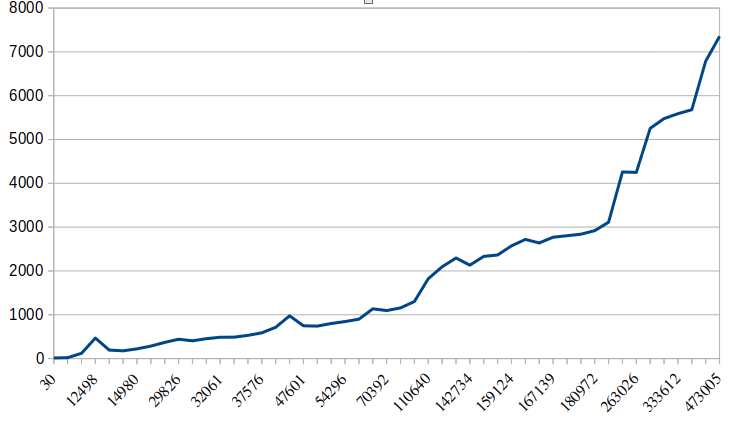
\includegraphics[width=\textwidth]{images/betoltesiido.png}
\caption{Modell betöltési idő grafikon.}
\label{fig:betolt}
\end{figure}

Modellek betöltési sebességét vizsgáltam a  \ref{fig:betolt}. grafikonon. A vízszintes tengelyen a modellek összes elemszáma (geometria csúcs, textúra koordináta, normál csúcs, lap elem) számok összesítése látható a függőleges tengelyen pedig a betöltési idő milliszekundumban. Az összehasonlítás textúra, modell kirajzolás, és az OBJ fájlon történő bármilyen változtatás nélkül történt.

A grafikonon jól látható hogy az idő növekedése közel exponenciális, tehát a modellek elemszámának növekedésének mértéke közel  arányos a beolvasáshoz szükséges idő nagyságával.
\bigskip
\Section{Modell betöltés sebességmérés az egyes részeken}
\bigskip
\begin{figure}[h]
\centering
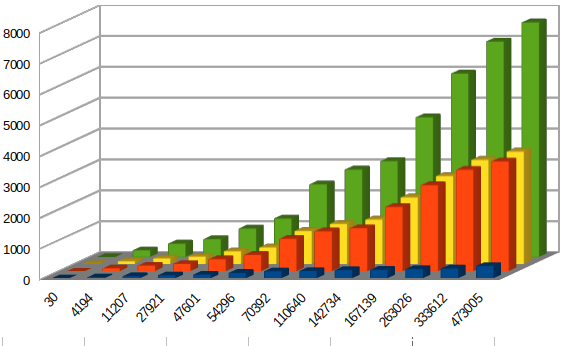
\includegraphics[width=\textwidth]{images/betoltesiido2.png}
\caption{Modell betöltési az egyes részeken grafikon.}
\label{fig:betolt2}
\end{figure}
\bigskip
\Aref{fig:betolt2}. diagramon látható modell betöltés a különböző részekre lebontva. Vízszintes tengelyen kapott helyet a modellek összes elemszáma. Függőleges tengelyen az idő milliszekundumban.
\begin{itemize}
\item Kék színnel különböző adatok feltöltéséhez szükséges tömbök lefoglalása.

\item Narancssárga színnel lett jelölve a különböző változók összeszámlálása.

\item Sárga színnel lett jelölve az adatok tényleges kiolvasása a fájlból.

\item Grafikonon zöld színnel lett jelölve modell teljes betöltésének ideje.
 \end{itemize}
\bigskip
\noindent Grafikonról  jól leolvasható, hogy a tömbök lefoglalása szinte jelentéktelen időt vesz igénybe a folyamat során. Változók összeszámlálása közel azonos időt vesz igénybe, mint a kiolvasás, ez azért van, mert mindkét folyamatnál végig kell menni a teljes OBJ fájl minden elemén. 
\Chapter{Összefoglalás}
A dolgozatban egy saját fejlesztésű objektum javító szoftver került elkészítésre és bemutatásra.

Az alkalmazás egy \texttt{obj\_corrector\_tool} nevű C nyelvű függvénykönyvtárban került megvalósításra.\\

Szakdolgozat témaválasztás során nem véletlenül választottam ezt a témát, egyetemi tanulmányaim alatt már rájöttem hogy a grafikus dolgok érdekelnek a leginkább az informatikában ezen belül is leginkább a 3D-s grafika.\\

Az adott feladatot miszerint egy saját javító szoftvert hozzak létre nagyon élveztem és sokat tanultam más szoftverek tesztelésétől elkezdve mind a tervezésen keresztül a megvalósításig végzett lépéseknél.\\

A program végül maga egyszerűségével maximálisan elérte a tervezetteket. Számomra egy mérföldkő, mivel ilyen komplex önálló feladatot az egyetemen még nem kellett létrehoznom.\\

Továbbfejlesztési lehetőségek közül talán a legfontosabb és egyben leginkább kézen fekvő, hogy ne csak háromszögeket és négyszögeket kezeljen a szoftver hanem ennél nagyobb csúcspont számú sokszögeket is emelett több javítási funkció implementálása . Nem utolsó sorban a teljes program tesztelés elkészítése a hibátlan működés érvényesítéséhez.


\clearpage

\addcontentsline{toc}{chapter}{Irodalomjegyzék}
\bibliographystyle{plain}
\bibliography{dolgozat.bib}

\newpage

\pagestyle{empty}

\noindent \textbf{\Large CD Használati útmutató}

\vskip 1cm

Ennek a címe lehet például \textit{A mellékelt CD tartalma} vagy \textit{Adathordozó használati útmutató} is.

Ez jellemzően csak egy fél-egy oldalas leírás.
Arra szolgál, hogy ha valaki kézhez kapja a szakdolgozathoz tartozó CD-t, akkor tudja, hogy mi hol van rajta.
Jellemzően elég csak felsorolni, hogy milyen jegyzékek vannak, és azokban mi található.
Az elkészített programok telepítéséhez, futtatásához tartozó instrukciók kerülhetnek ide.

A CD lemezre mindenképpen rá kell tenni
\begin{itemize}
\item a dolgozatot egy \texttt{dolgozat.pdf} fájl formájában,
\item a LaTeX forráskódját a dolgozatnak,
\item az elkészített programot, fontosabb futási eredményeket (például ha kép a kimenet),
\item egy útmutatót a CD használatához (ami lehet ez a fejezet külön PDF-be vagy MarkDown fájlként kimentve).
\end{itemize}


\end{document}